\documentclass[11pt,letter]{article}
\usepackage[top=1.00in, bottom=1.0in, left=1.1in, right=1.1in]{geometry}
\usepackage{graphicx} % Required for inserting images
\usepackage{xcolor} 
\definecolor{Accent}{HTML}{bd2b00} 
\usepackage{natbib}
\usepackage{gensymb}
\usepackage{hyperref}
\hypersetup{colorlinks,citecolor = Accent, linkcolor = Accent,urlcolor = Accent, breaklinks=true}
\usepackage{cleveref}
\usepackage[labelfont=bf]{caption}
\bibliographystyle{amnat}

\RequirePackage[labelfont={bf,sf},%
                font={small, sf}]{caption}


\title{Solstice optimizes thermal growing season}

\author{Victor, Lizzie}
\date{Aug.-Nov. 2024}

\begin{document}

\maketitle

%\begin{enumerate}

%\item New (recent) exciting findings! Solstice, "\emph{celestial starting gun}"\\
%(Bad) consequences for climate change forecasting: plants are stuck? \\
% $\rightarrow$ But leave an open question: why solstice?
%emw11Dec: I would remove the word 'phenology' from the paper, since some will not know it and we don't use it much (three times I think?). Alternatives are: life history events or growth and reproductive events (or delete it when not critical). I tossed in various ones, but feel free to change! 
Plants generally use environmental cues to adjust the timing of major growth and reproductive events in response to variability within and between years. While we often know the proximate triggers---such as temperature and photoperiod---the larger mechanisms behind these cues remain largely unknown for many events \citep{Chuine2017}, leaving a critical gap in our understanding of how plants will respond and adapt to future climates.
% Gao2024: "we do not know when plants start responding to temperatures, what range of temperatures influences spring phenology, and how and why these controls vary by species or climate conditions"

Recently, summer solstice has been proposed as a universal trigger to modulate cues and initiate key physiological processes \citep{Zohner2023, Journe2024}---an idea that builds on earlier suggestions of solstice-driven control of tree growth \citep{Rossi2006}. 
Plants may rely on the solstice as a signal to initiate the shift from growth to tissue maturation before winter and to prepare for reproduction in the following year through flower bud differentiation \citep{Rossi2006, Zohner2023, Journe2024}.
% JDavies: "You never really explain what this switch is - what are plants doing?"
% DBuonaiuto: "I think this paragraph could use another sentence or two explaining the proposed physiological mechanism about how the soltice modulates cues."
This proposed photoperiod switch, if correct, could reshape predictions of forest responses to climate change. It would also suggest a fundamental new mechanism for how plants sense photoperiod \citep{Gendron2023}. 
Using a fixed date like the solstice as a cue, however, could limit plasticity and become less suitable 
% JDavies: "what exactly becomes less suitable?"
in a warmer future climate \citep{Bonamour2019}. 
This may in turn drive forest declines, with significant implications for carbon storage \citep{green2022limits}, and thus raises important questions about the suitability for plants to rely on the solstice. 

% \item Plants need to balance transition to events at best moment vs end-of-season constraint, i.e. choose when to transition without full info\\
% $\rightarrow$ Need to optimize predictions!
The timing of major plant transitions---such as start of growth with leafout---should match development states with fitness opportunities, given no other constraints. In most environments, this involves a trade-off between %increased fitness % changed based on JDavies comment: "typically, when we refer to 'fitness' it includes these tradeoffs, perhaps better to refer to 'increased opportunity for growth"?"
increased opportunity for growth and reproduction
(e.g. a longer window for growth) and increased susceptibility to climatic and biotic risks (e.g. a higher exposition to late frosts). Because plants cannot know these exact opportunities and risks in advance, they should rely on the most informative cues to accurately anticipate environmental conditions and optimize their chances for growth and reproduction \citep{Chevin2015, Bonamour2019}.

% \item (Thermal) $GDD$ as a critical integrator\\
% Critical both to crops and wild plants\\
%Plants want to grow as much as possible during warm years, and benefit from warm years to set many flowers (flower differentiation?)
In particular, it is well established that plants respond primarily to integrated climate forcing, often measured as the accumulation of warm temperatures, in a given range---where metabolism is sufficient---and over a given period \citep[growing degree-days or GDD;][]{Chuine2017}.
This heat accumulation is a key factor in development and growth processes of both crops \citep[e.g.][]{Cross1972} and wild plants \citep[e.g.][]{Hunter1992}. The number of GDD accumulated throughout the season directly impacts how quickly cells elongate to form new organs and how quickly a plant progresses through growth stages. Plants are thus expected to take full advantage of warmer years (with a high GDD accumulation) to maximize growth and set more flowers for the following season \citep{larcher1980}. 

% \item Given $GDD$ is so important, plants should thus transition into events when they can best predict $GDD_{total}$ within growing season -- while still having enough time/energy \emph{to do what they need to do}
Given the importance of GDD, plants should ideally time their transitions when their ability to predict the total GDD within the growing season is high while still having enough potential thermal energy to complete essential growth and reproductive processes. This trade-off means that there should be an optimal period when plants have accumulated enough GDD
% JDavies: "it seems it is not so much about how much GDD they have accumulated but rather how far through the season they are - how much more they can invest in growth before they have to switch to reproduction, right?"
to reliably predict the total GDD by the end of the year---\emph{environmental predictability}, while enough GDD still remains---which we call \emph{growth potential}. Here, we define environmental predictability based on how well GDD accumulated by a day ($d$) predicts the total GDD 
% JDavies: "This is a (The) critical part of your analysis, and I think this definition needs better justification/explanation."
% something like: i.e. It directly relates to how plants accumulate information and gain predictive power through the season?
each year (measured as the $R^2$ of a linear regression across years using 1 January to start accumulation). This measure directly relates to how plants accumulate information and gain predictive power through the season. % added this sentence to answer Jonathan comment
Growth potential, on the other hand, is defined as the remaining GDD on day $d$ (see Supplementary Methods and Supplementary Figure S1). %emw11Dec: please check if my edits still present this correctly ... 
This simple 
% definition 
trade-off
allows us to examine which window in the season appears optimal for plants to maximize growth and development while minimizing risks.
% JDavies: "explain which window this is - why should plants switch at the solstice just because it is where they have optimal predictive ability regarding rest of the season?"
% DBuonaiuto: "Can you end this paragraph with a prediction of some kind? Basically just give the readers a bit more information about what they should be looking for."
% something like: thus, the period where... to work

\begin{figure}[h]
\centering
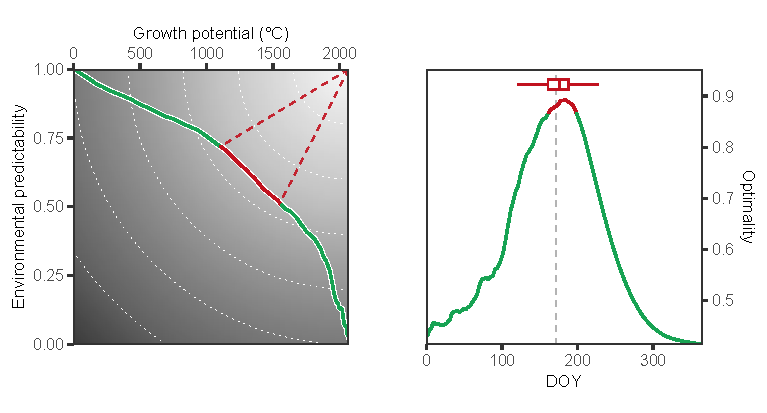
\includegraphics{global_optimality.pdf}
\vspace*{-0.5cm}
\caption{\textbf{Solstice marks the average optimal trade-off between environmental predictability and growth potential across Europe (1951-2020).} In the left panel, environmental predictability measures how well GDD by a given day predicts total yearly GDD ($R^2$ of a linear regression across years), while growth potential represents the remaining GDD from that day onward. In the right panel, optimality is based on the Euclidean distance from the (unattainable) perfect point where both predictability and growth potential are maximized (illustrated by the red dashed lines and the gray gradient in the left panel). The red sections of the green curves represent days where optimality falls within the 90th percentile (i.e. top 10\% most optimal days). GDD range was defined between 5\degree C and 35\degree C (see Figure S2 for 0-40\degree C).} 
\label{fig:globaloptimality}
\end{figure}

% \item We found this optimal point in Europe to be the solstice(ish)\\
% \begin{enumerate}
%     \item If this true widely, then evolution towards an universal solstice trigger could make sense, right? 
%     \item But our results also suggest we cannot teasee appart solstice and thermal optimum-predictability cue
% \end{enumerate}
We found the optimal period to be near the summer solstice (\Cref{fig:globaloptimality}). Averaging across all of Europe, solstice appears as a critical juncture for the optimization of both environmental predictability and growth potential.
% JDavies: "I think you need to explain this better, if plants want to optimise growth potential they should just keep on growing ..."
If this specific day indeed represents a broad-scale optimum across different climatic conditions, plant evolution towards a universal solstice trigger could make sense---especially since this optimum appears stable over the Holocene (Supplementary Figure S3). %emw11Dec: Nice additional analysis!
% It could act as a reliable marker for when a plant has likely accumulated the right amount of GDD. 
%emw11Dec: I don't love 'the right amount' ... we could maybe delete the sentence or change to: It could thus act as a reliable marker of each year's expected GDD before too late in the season. OR ... start a new paragraph as I suggest here ...
% Our results also suggest it is challenging to disentangle the influence of the solstice from that of a thermal optimum cue.

Our results suggest solstice could act as a reliable marker but also highlight that it is challenging to disentangle the influence of the solstice from that of a thermal optimum cue. %emw11Dec: We may need to spell this out more clearly than your sentence does? 
We show that solstice trades-off environmental predictability and growth potential, but given our metrics are based on a thermal season, plants may equally use thermal cues for the same outcome.
% DBuonaiuto: "Can you say this a bit more clearly? Walk us through what you mean here"
% 
% does solstice coincide with the period of highest thermal energy in temperate regions? Peak of daily GDD is rather after solstice...
Plants could also rely on a combination of both solstice and thermal cues to optimize growth and reproductive timing---which could provide greater signal robustness to environmental change through partial redundancy between cues \citep{Bonamour2019}.
Alternatively, this overlap could simply represent an emergent property of the climate system that plants don't necessarily use as a cue, since it would be costly for plants to closely track two different signals---i.e. to encode and decode both thermal and daylength information within their cells. 

% \item Supporting this we found important variation over space (and time?)
%emw11Dec: I don't think cautionary is what we want ... depends on what you mean above. (If we need to toss the coincidence point above then I think we need to set up more in the end of the previous paragraph how this evolution would happen -- and at what scales perhaps.)
Supporting the hypothesis of an alternative cue to the solstice, our results reveal substantial variation in the optimal timing across Europe (\Cref{fig:localoptimality}). In warmer southern Europe, plants reach an optimum earlier in the season, whereas in northern regions, cooler temperatures delay this timing beyond the solstice. 
% JDavies: "is there some way you can show plants in these regions don't use solstice?  I think I mentioned this to Lizzie earlier, but it would be great if you could show whether plants that were poorly predicted by solstice (in Zhoner et al. 2023) fall in regions where solstice is a poor predictor!"
This regional variability suggests that plants should likely 
%be partially adapted to their local climates---and especially to how GDD accumulate in their specific environment 
rely on cues that allow for a plastic response in their specific environment. 
From a parsimonious perspective, tracking primarily GDD-related cue might be more straightforward and aligned with the actual energy a plant needs to grow and reproduce---i.e. the cue would be sampled from a variable directly used by the plant.
 % (= directly linked to metabolic processes) i.e. the cue is sampled from a variable directly use by the plant
%emw11Dec: Recommend with stick with photoperiod or daylength across whole paper unless we're making an important distinction. 
Whereas tracking the solstice is likely more complex. Indeed, plants would need to sense not just the daylength but also the variation in the rate of change of day length over time---essentially, the second derivative.
% more directly beneficial for the plant?
% What would be the benefit to have a separate mechanism, with the risk of a potential redundancy of tracking both the solstice and thermal cues? (but which thermal cue to track the optimal period?) => increase robustness of the signal with  partial redundancy bewteen cues


% Maybe we need to talk more about photoperiod cue sensing? What is known ("not a new result" Isabelle...) => make a paragraph?
% second derivative sensing seems unlikely, but we know photoperiod can be important?
% what could be the benefit of tracking photoperiod => synchronize populations broadly?
% if plants don't use solstice or if they don't use photoperiod, which cue(s) they need to track to understand that it is the optimal period, ? Temperature (and daily GDD accumulation) peaks after the optimum, so it should be something else?
% Does using solstice will prevent adaptative plasticity in future climate, ie plants could be "locked in a solstice response" (and mention supp figure with CMIP6 projections?)
% + "photosynthetic capacity peaks just after summer solstice and declines with decreasing photoperiod, before air temperatures peak" https://www.pnas.org/doi/10.1073/pnas.1119131109#fig02
% "In the most extreme cases, a new environment is generating a signal similar to a previously known cue, but completely uncorrelated with both the original cue and the environment of selection."


% \begin{enumerate}
%     \item critical need for experiments to disentangle daylength vs temp.
%     \item researchers need to more clearly test for (i) trends estimated at local scale across gradient and (ii) how they scale up to (sub)continental/global scales
% \end{enumerate}
Disentangling the role of the solstice as a cue for major growth and reproductive transitions is challenging, as plants have already started accumulating GDD several months before the solstice.
Complex natural correlations in environmental data may generate spurious results \citep[e.g.][]{Gao2024}, challenging us to test predictions from multiple avenues. % "inherent correlations in climate in regions that the field does not fully understand/incorporate"
Future research should explore which thermal cues might allow plants to track the optimal period, how these compare to a solstice-based cue, and whether they remain reliable in future climates (Supplementary Figures S4 and S5).
% as daily GDD accumulation peak after solstice suggests the need for an alternative cue...?
To address this requires carefully designed experiments that decouple natural covariation between temperature and photoperiod  \citep{Buonaiuto2023} and integrate new understanding of the multiple ways plants sense daylength \citep{wang2024plants}.  
%emw11Dec: Hmm, I suspect there is a Korner or Basler paper we could cite instead of Dan's paper? 
%vvdm17Dec: do you have a specific paper in mind? this one: https://doi.org/10.1093/treephys/tpu021 ? (even though the focus is not on the covariation of temperature and photoperiod?)
Beyond small-scale experiments, understanding local-scale trends and how they scale up to subcontinental scales could help inform what trends plants may leverage to predict their environments over time. 
Ultimately, a better understanding of how plant responses to photoperiod and temperature vary regionally will help clarify broader synchrony patterns.
% =>  and finally: inform phenological models, allowing researchers to build more accurate predictions by incorporating the specific cues plants use to trigger growth
% JDavies: "reference to 'synchrony' comes out of nowhere ..."

\begin{figure}[h]
% \centering
\hspace*{-1.2cm}
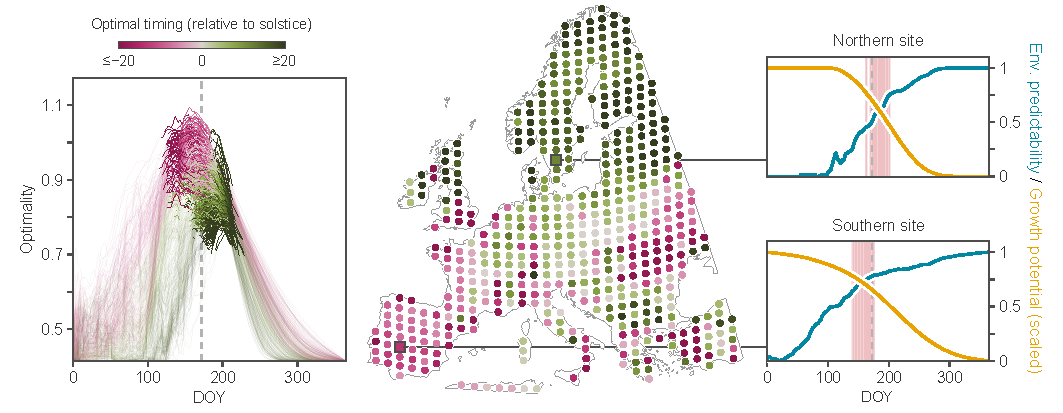
\includegraphics{local_optimality_alt.pdf}
\vspace*{-0.7cm}
\caption{\textbf{Variation in optimal timing reflects different climatic conditions across Europe (1951-2020).} On the left panel, each curve shows the evolution of optimality for a given site. Sites are sampled on a regular grid across Europe, as shown on the central map. Colors indicate the timing---relative to the solstice---of the median optimal day. The two panels on the right show the trade-off between environmental predictability and growth potential (scaled to $[0,1]$) for two different sites. Days considered as optimal are highlighted in red.}
\label{fig:localoptimality}
\end{figure}

%\end{enumerate}
\clearpage
\bibliography{synchrony}

\end{document}
